\documentclass[border=5pt]{standalone}
\usepackage{tikz}
\usepackage{pgfplots}
\pgfplotsset{compat=1.17}
\usepackage{amsmath}

\begin{document}
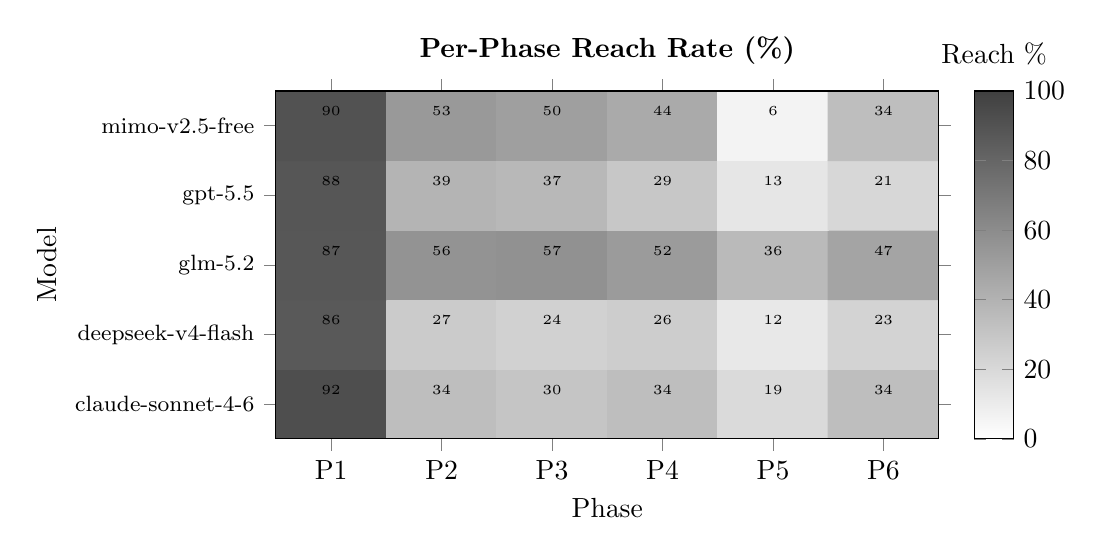
\begin{tikzpicture}
\begin{axis}[
    width=10cm,
    height=6cm,
    colormap={hexmap}{color=(white) color=(black!75)},
    colorbar,
    colorbar style={
        title={Reach \%},
        ytick={0,20,40,60,80,100},
    },
    point meta min=0,
    point meta max=100,
    xtick={0,1,2,3,4,5},
    xticklabels={P1,P2,P3,P4,P5,P6},
    ytick={0,1,2,3,4},
    yticklabels={claude-sonnet-4-6, deepseek-v4-flash, glm-5.2, gpt-5.5, mimo-v2.5-free},
    xtick align=outside,
    ytick align=outside,
    xlabel={Phase},
    ylabel={Model},
    title={\textbf{Per-Phase Reach Rate (\%)}},
    enlargelimits=false,
    axis on top,
    nodes near coords={\pgfmathprintnumber[precision=0]{\pgfplotspointmeta}},
    every node near coord/.append style={font=\tiny, /pgf/number format/assume math mode=true},
    y tick label style={font=\footnotesize},
]
\addplot[
    matrix plot*,
    mesh/cols=6,
    point meta=explicit,
] coordinates {
    % claude-sonnet-4-6 (y=0)
    (0,0)[92] (1,0)[34] (2,0)[30] (3,0)[34] (4,0)[19] (5,0)[34]
    % deepseek-v4-flash-free (y=1)
    (0,1)[86] (1,1)[27] (2,1)[24] (3,1)[26] (4,1)[12] (5,1)[23]
    % glm-5.2 (y=2)
    (0,2)[87] (1,2)[56] (2,2)[57] (3,2)[52] (4,2)[36] (5,2)[47]
    % gpt-5.5 (y=3)
    (0,3)[88] (1,3)[39] (2,3)[37] (3,3)[29] (4,3)[13] (5,3)[21]
    % mimo-v2.5-free (y=4)
    (0,4)[90] (1,4)[53] (2,4)[50] (3,4)[44] (4,4)[6] (5,4)[34]
};
\end{axis}
\end{tikzpicture}
\end{document}
